\documentclass[12pt, a4paper]{report}
\usepackage[utf8]{inputenc}
\usepackage[english, russian]{babel}

\usepackage{graphicx}
\usepackage{listings}
\usepackage{color}

\usepackage{amsmath}
\usepackage{pgfplots}
\usepackage{url}
\usepackage{flowchart}
\usepackage{tikz}
\DeclareGraphicsExtensions{.pdf,.png,.jpg,.svg}
\usetikzlibrary{shapes, arrows}

\usepackage{pgfplotstable}

\renewcommand\contentsname{Содержание}

\usepackage{geometry}
\geometry{left=3cm}
\geometry{right=1cm}
\geometry{top=2cm}
\geometry{bottom=2cm}

\lstset{ %
language=C++,                 % выбор языка для подсветки (здесь это С)
basicstyle=\small\sffamily, % размер и начертание шрифта для подсветки кода
numbers=left,               % где поставить нумерацию строк (слева\справа)
numberstyle=\tiny,           % размер шрифта для номеров строк
stepnumber=1,                   % размер шага между двумя номерами строк
numbersep=-5pt,                % как далеко отстоят номера строк от         подсвечиваемого кода
backgroundcolor=\color{white}, % цвет фона подсветки - используем         \usepackage{color}
showspaces=false,            % показывать или нет пробелы специальными     отступами
showstringspaces=false,      % показывать или нет пробелы в строках
showtabs=false,             % показывать или нет табуляцию в строках
frame=single,              % рисовать рамку вокруг кода
tabsize=2,                 % размер табуляции по умолчанию равен 2 пробелам
captionpos=t,              % позиция заголовка вверху [t] или внизу [b] 
breaklines=true,           % автоматически переносить строки (да\нет)
breakatwhitespace=false, % переносить строки только если есть пробел
escapeinside={\%*}{*)},   % если нужно добавить комментарии в коде
keywordstyle=\color{blue}\ttfamily,
stringstyle=\color{red}\ttfamily,
commentstyle=\color{green}\ttfamily,
morecomment=[l][\color{magenta}]{\#},
columns=fullflexible }

\usepackage{titlesec}
\titleformat{\chapter}[hang]{\LARGE\bfseries}{\thechapter{.} }{0pt}{\LARGE\bfseries}
\titleformat*{\section}{\Large\bfseries}
\titleformat*{\subsection}{\large\bfseries}

\begin{document}

    \begin{titlepage}

        \begin{center}
            \Large
            {\sl Государственное образовательное учреждение высшего профессионального образования\\
            {\bf«Московский государственный технический университет имени Н.Э. Баумана»\\
				(МГТУ им. Н.Э. Баумана)}}
            \vspace{3cm}

			{\scshape\LARGE Лабораторная работа №4 \par}
			\vspace{0.5cm}	
			{\scshape\LARGE по курсу «Анализ алгоритмов» \par}
			\vspace{1.5cm}
			{\huge\bfseries Многопоточность \par}
			\vspace{2cm}
			\Large Выполнил: Тимонин А.С., гр. ИУ7-52Б\\
			\vspace{0.5cm}
			{\Large Преподаватели: Волкова Л.Л., Строганов Ю.В.}
		
			\vfill
			\Large \textit {2019 г.}
            
        \end{center}

    \end{titlepage}
	
	\tableofcontents

	\chapter*{Введение}
	\addcontentsline{toc}{chapter}{Введение}
	
	\vspace{-0.5cm}\hspace{0.6cm}Многопоточность (как доктрину программирования) не следует путать ни с многозадачностью, ни с многопроцессорностью, несмотря на то, что операционные системы, реализующие многозадачность, как правило, реализуют и многопоточность. Смысл многопоточности - квазимногозадачность на уровне одного исполняемого процесса[2].
		
	\vspace{0.3cm}В данной работе требуется рассмотреть алгоритм Винограда для умножения матриц в однопоточной и многопоточной реализациях, а также провести сравнительный анализ.
	
		\vspace{0.3cm}Цель работы: изучение многопоточности и получение практики на примере алгоритма Винограда для перемножения матриц.
	
		\vspace{0.3cm}Задачи работы:
	\begin{enumerate}
		\item Разработка и реализация алгоритмов.
		\item Исследование временных затрат алгоритма.
		\item Описание и обоснование полученных результатов.
	\end{enumerate}
	

    \chapter{Аналитический раздел}
    
   	\vspace{-0.5cm}\hspace{0.6cm}В данном разделе будет описан алгоритм Винограда для перемножения матриц.
   	
   	
	\section{Алгоритм Винограда}
	
	Алгоритм Винограда это модифицированная версия классического алгоритма, где часть процессов высчитывается заранее. Эти вычисления позвовлят разбить вычисления алгоритма на потоки. Пусть есть две матрицы A и B размеров nxk, kxm соответственно. Тогда результатом перемножения этих двух матриц будет матрица C размера nxm \ref{for:lol1}.
	
	\begin{equation}
	A_{nk} * B_{km} = C = \begin{pmatrix}
		c_{11} & c_{12} & \cdots & c_{1m} \\
		c_{21} & c_{22} & \cdots & c_{2m} \\         
		\vdots & \vdots & \ddots & \vdots \\
		c_{n1} & c_{n2} & \cdots & c_{nm} \\
	\end{pmatrix}
	\label{for:lol1}
	\end{equation}
	
	Если посмотреть на результат умножения двух матриц, то можно заметить, что каждый элемент в нем представляет собой скалярное произведение соответствующих строки и столбца исходных матриц. Также, такое умножение позволяет сделать предварительную обработку заранее \cite{Volkova}
	
	Пусть два вектора $$V = (v1, v2, v3, v4), $$
	 
	$$W = (w1, w2, w3, w4)$$
	
	Тогда их скалярное произведение равно: 
	$$V * W = v1w1 + v2w2 + v3w3 + v4w4$$
	Это равенство можно переписать в виде: 
	$$V * W = (v1 + w2)(v2 + w1) + (v3 + w4)(v4 + w3) - 
	v1v2 - v3v4 - w1w2 - w3w4$$
	

	\section{Многопоточность}
	
	\hspace{0.6cm}Существуют зеленые и нативные потоки. Зеленые потоки - это потоки выполнения, управление которыми вместо операционной системы выполняет виртуальная машина. Программа написанная на языке, поддерживающим зеленые потоки, только эмитирует многопоточность. 
	
	\vspace{0.3cm}На многоядерных процессорах реализация нативных потоков может автоматически назначать работу нексольким процессорам, а реализация зеленых потоков не может назначить работу нескольким процессорам.
	
	\vspace{0.3cm}Поток выполнения - наименьшая единица обработки, исполнение которой может быть назначено ядром операционной системы. Реализация потоков выполнения и процессов в разных операционных системах отличается друг от друга, но в большинстве случаев поток выполнения находится внутри процесса. Несколько потоков выполнения могут существовать в рамках одного и того же процесса и совместно использовать ресурсы, такие как память, тогда как процессы не разделяют этих ресурсов[1]
	
	\section{Вывод}
	
	В данном разделе был описан алгоритм Винограда перемножени матриц.
	

	\chapter{Конструкторский раздел}
	
	\vspace{-0.6cm}\hspace{0.6cm} В данном разделе будет приведена блок-схема алгоритма Винограда для перемножения матриц, описано для каких частей алгоритма выделялись потоки, и каким образом это было реализовано.
	
	\section{Разработка алгоритмов}
	
	\hspace{0.6cm}В данном пункте представлена реализация алгоритма Винограда на рис. \ref{scheme}. 
	
	\newpage
	
	\begin{figure}[ht!]
		\label{scheme}
		\centering
		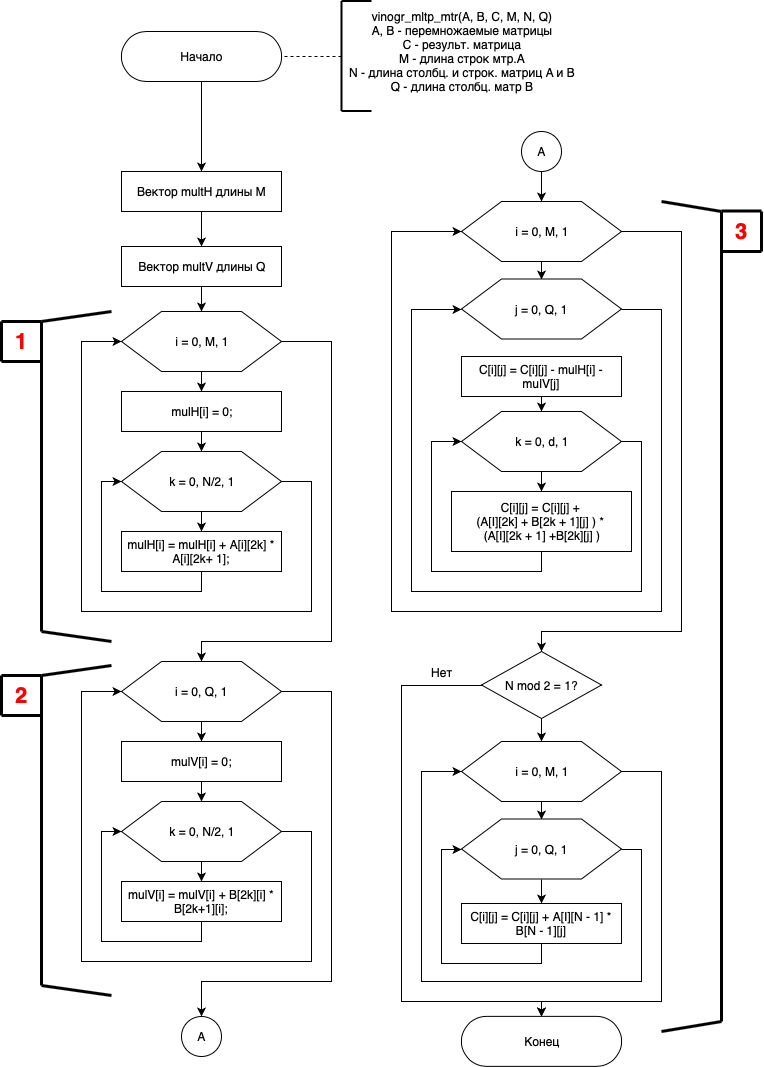
\includegraphics[scale=0.6]{scheme.png}
		\caption{Схема алгоритма Винограда}
	\end{figure}



	\newpage
	
	Для реализации многопоточной версии алгоритма можно выделить 4 основные части
	
	\begin{enumerate}
		\item Создание и инициализация MulH.
		\item Создание и инициализация MulV.
		\item Основные и дополнительные(для входных матриц нечетной размерностей) вычисления матрицы произведения.
	\end{enumerate}

	Части 1, 2 разбиваются по потокам. Поток для 3 части не выделяется, пока не выполнятся 1 и 2 части.

	
	\section{Вывод}
	В данном разделе была приведена схема алгоритма, было описано каким образом выделялись потоки в реализованном алгоритме Винограда.
	
	\newpage
	
	\chapter{Технологический раздел}
	\vspace{-0.5cm}В данном разделе будут рассмотренны требования к разрабатываемому программному обеспечиванию, средства, использованные в процессе разработки для реализации поставленных задач, а также представлены листинги кода программы.
	
	\section{Требования к программному обеспечению}
	Программное обеспечивание должно реализовывать алгоритм Винограда для перемножения матриц в однопоточной и многопоточных реализациях.
	
	\section{Средства реализации}
	\hspace{0.6cm}Для выполнения поставленной задачи был использован язык программирования С++. Среда для разработки XCode. Для измерения процессорного времени была взята функция duration из библиотеки chrono.
	
	\vspace{0.2cm}Версия компилятора C++: GNU++14 [-std=gnu++14]
	
	
	\section{Листинг кода}
	\hspace{0.6cm}На основе схема, приведенной в конструкторском разделе, в соответствии с указанными требованиями к реализации с использованием языка С++ было разработано программное обеспечение, содержащее реализации выбранных алгоритмов. В данном пункте приведен листинги \ref{code1}-\ref{code2} реализации алгоритма.

	\begin{lstlisting}[label=code1,caption=Реализация алгоритма Винограда]
	void Vinograd_n_thread(matrix_type &a, matrix_type &b, matrix_type &c, int n)
	{
	vector<int> row(a.n);
	vector<int> column(b.m);
	
	vector<thread> threads;
	
	unsigned int n1 = a.n / 2;
	zeroing(c.matrix, c.n, c.m);
	
	double length_part = (double) a.n / n;
	if (length_part < 1) {
	length_part = 1;
	}
	
	for (int i = 0; i < a.n; i++) {
	row.push_back(0);
	}
	for (int i = 0; i < b.m; i++) {
	column.push_back(0);
	}
	
	thread thr_mulH(create_mulH, ref(a.matrix), ref(row), 0, ref(a.n), ref(a.m));
	thread thr_mulV(create_mulV, ref(b.matrix), ref(column), 0, ref(b.m), ref(b.n));
	
	thr_mulH.join();
	thr_mulV.join();
	
	for (int i = 1; i <= n; i++) {
	threads.push_back(thread(calculate1, ref(a), ref(b), ref(c), ref(row), ref(column), (a.n * (i - 1)) / n, (a.n * i) / n));
	}
	
	for (int i = 0; i < threads.size(); ++i) {
	if (threads[i].joinable()) {
	threads[i].join();
	}
	}
	}
	
	\end{lstlisting}

	\begin{lstlisting}[label=code2,caption=Основные вычисления для многопоточной реализации алгоритма Винограда]
	void create_mulH(int **&A, vector <int>& row, const unsigned int &M_start, const unsigned int &M_end, const unsigned int &N)
	{
	
	for (unsigned i = M_start; i < M_end; i++) {
	//cout << this_thread::get_id()<< endl;
	for (unsigned k = 0; k < N / 2; k++) {
	row[i] += A[i][2 * k] * A[i][2 * k + 1];
	}
	}
	}
	
	void create_mulV(int **&B, vector <int>& column, const unsigned int &Q_start, const unsigned int &Q_end, const unsigned int &N)
	{
	
	for (unsigned i = Q_start; i < Q_end; i++) {
	//cout << this_thread::get_id()<< endl;
	for (unsigned k = 0; k < N / 2; k++) {
	column[i] += B[2 * k][i] * B[2 * k + 1][i];
	}
	}
	}
	
	void calculate(int **&A, int **&B, int **&C, vector <int> &row, vector <int> &column, const unsigned int &M, const unsigned int &N, const unsigned int &Q)
	{
	for (unsigned i = 0; i < M; i++)
	for (unsigned j = 0; j < Q; j++) {
	if (N % 2 == 0)
	C[i][j] = -row[i] - column[j];
	else
	C[i][j] = -row[i] - column[j] + A[i][N - 1] * B[N - 1][j];
	
	for (unsigned k = 0; k < N / 2; k++) {
	C[i][j] = C[i][j] + (A[i][k << 1] + B[k << 1 | 1][j]) *
	(A[i][k << 1 | 1] + B[k << 1][j]);
	}
	}
	
	}
	
	void calculate1(matrix_type &a, matrix_type &b, matrix_type &c, vector <int> &row, vector <int> &column, const unsigned int n_start, unsigned int n_end)
	{
	int sum = 0;
	
	for (unsigned i = n_start; i < n_end; i++) {
	//cout << this_thread::get_id()<< endl;
	for (unsigned j = 0; j < b.m; j++) {
	
	sum = -row[i] - column[j];
	
	for (unsigned k = 0; k < a.m / 2; k++) {
	sum += (a.matrix[i][2*k] + b.matrix[2*k+1][j]) *
	(a.matrix[i][2*k+1] + b.matrix[2*k][j]);
	}
	
	if (a.m % 2 == 1)
	sum += a.matrix[i][a.m - 1] * b.matrix[b.n - 1][j];
	
	c.matrix[i][j] = sum;
	}
	}
	
	}
	
	\end{lstlisting}

	\newpage

	\section{Вывод}
	В данном разделе были рассмотрены требования к разрабатываемому программному обеспечению, средства, использованные в процессе разработки, а также был представлены листинги кода реализации алгоритма Винограда.

			
	\chapter{Экспериментальный раздел}
	
	\vspace{-0.6cm}\hspace{0.5cm}В данном разделе будет приведено экспериментальное исследование временных затрат разработанного программного обеспечения, вместе в подробным сравнительным анализом реализованных алгоритмов на основе экспериментальных данных.
	
	\section{Сравнительный анализ}
	
	\hspace{0.6cm}Замеры времени выполнялись на квадратных матрицах размеров от 100х100 до 1000х1000 с интервалом в 100 элементов. Также замеры времени проводились над квадратными матрицами нечетной размерностью  от 101х101 до 1001х1001 с шагом 100. В табл. \ref{table1}-\ref{table2} и рис. \ref{pic1}-\ref{pic2} представлены результаты замеров времени в тактах.
	
	\vspace{0.3cm}Все замеры проводились на процессоре 1,4 GHz Intel Core i5 с памятью 8 ГБ 2133 MHz LPDDR3.
	
	\begin{table}[ht!]
		\caption{Сравнение времени работы однопоточной и многопоточной версий алгоритма в единицах измерения библиотеки chrono}
		\label{table1}
		\begin{center}
			\begin{tabular}{|c|c|c|c|c|c|c|}
				\hline
				\bf{Размерность матриц} & \bf{Поток 1} & \bf{Поток 2} & \bf{Поток 3} & \bf{Поток 4} &\bf{Поток 5} & \bf{Поток 6} \\\hline
				
				$100$ & $4$ & $2$ & $1$ & $1$ & $1$ & $1$ \\ \hline
				
				$200$ & $36$ & $17$ & $7$ & $6$ & $6$ & $6$\\\hline
				
				$300$ & $128$ & $56$ & $36$ & $35$ & $27$ & $27$\\\hline
				
				$400$ & $334$ & $165$ & $111$ & $89$ & $90$ & $77$\\\hline
				
				$500$ & $590$ & $331$ & $205$ & $176$ & $161$ & $148$\\\hline
				
				$600$ & $932$ & $535$ & $369$ & $279$ & $250$ & $241$\\\hline
				
				$700$ & $1504$ & $857$ & $591$ & $505$ & $465$ & $423$\\\hline
				
				$800$ & $2329$ & $1261$ & $815$ & $710$ & $731$ & $675$\\\hline
							
			    $900$ & $3808$ & $2818$ & $1570$ & $1166$ & $1131$ & $1084$ \\\hline
				
				$1000$ & $10691$ & $4392$ & $2743$ & $2169$ & $1816$ & $1529$\\\hline
			\end{tabular}
		\end{center}
	\end{table}

	\newpage

	\begin{figure}[ht!]
		\label{pic1}
		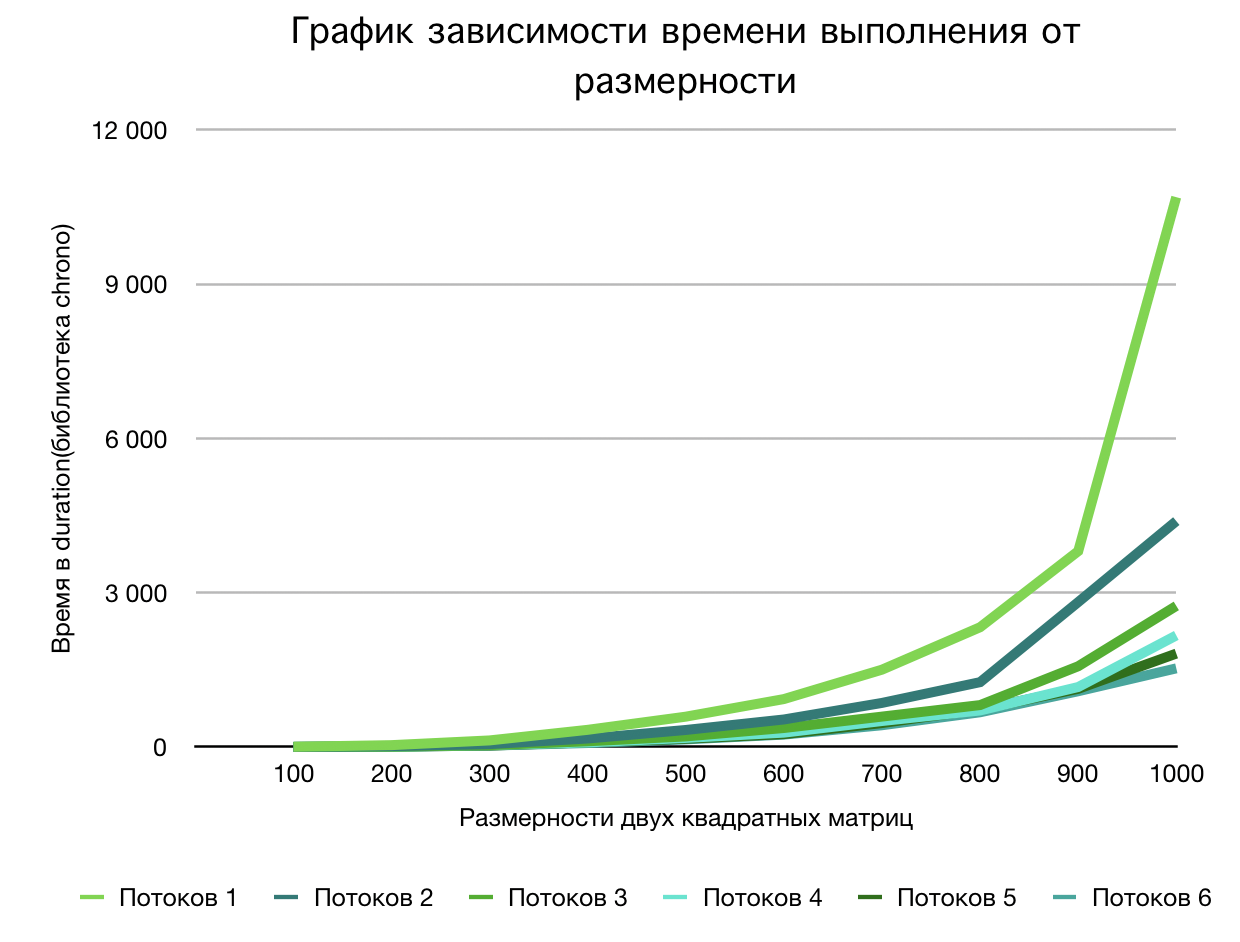
\includegraphics[scale=0.75]{table1}
		\caption{График зависимости времени работы однопоточной и многопоточных версий 	алгоритма для четной размерности матриц}
		\label{fig:image}
	\end{figure}

	\newpage

\begin{table}[ht!]
	\caption{Сравнение времени работы однопоточной и многопоточной версий алгоритма в единицах измерения библиотеки chrono}
	\label{table2}
	\begin{center}
		\begin{tabular}{|c|c|c|c|c|c|c|}
			\hline
			\bf{Размерность матриц} & \bf{Поток 1} & \bf{Поток 2} & \bf{Поток 3} & \bf{Поток 4} & \bf{Поток 5} & \bf{Поток 6} \\\hline
			
			$101$ & $4$ & $2$ & $1$ & $1$ & $1$ & $1$\\\hline
			
			$201$ & $24$ & $15$ & $7$ & $11$ & $7$ & $7$\\\hline
			
			$301$ & $116$ & $62$ & $37$ & $26$ & $31$ & $30$\\\hline
			
			$401$ & $320$ & $153$ & $111$ & $86$ & $84$ & $75$\\\hline
			
			$501$ & $531$ & $306$ & $209$ & $163$ & $150$ & $142$\\\hline
			
			$601$ & $993$ & $492$ & $333$ & $260$ & $249$ & $242$\\\hline
			
			$701$ & $1487$ & $853$ & $556$ & $455$ & $556$ & $428$\\\hline
			
			$801$ & $2482$ & $1154$ & $850$ & $699$ & $729$ & $643$\\\hline
			
			$901$ & $6480$ & $2810$ & $1562$ & $1093$ & $1175$ & $1362$ \\\hline
			
			$1001$ & $8949$ & $3892$ & $2645$ & $2179$ & $2260$ & $2054$\\\hline
		\end{tabular}
	\end{center}
\end{table}

	%\newpage
	
	\begin{figure}[ht!]
		\label{pic2}
		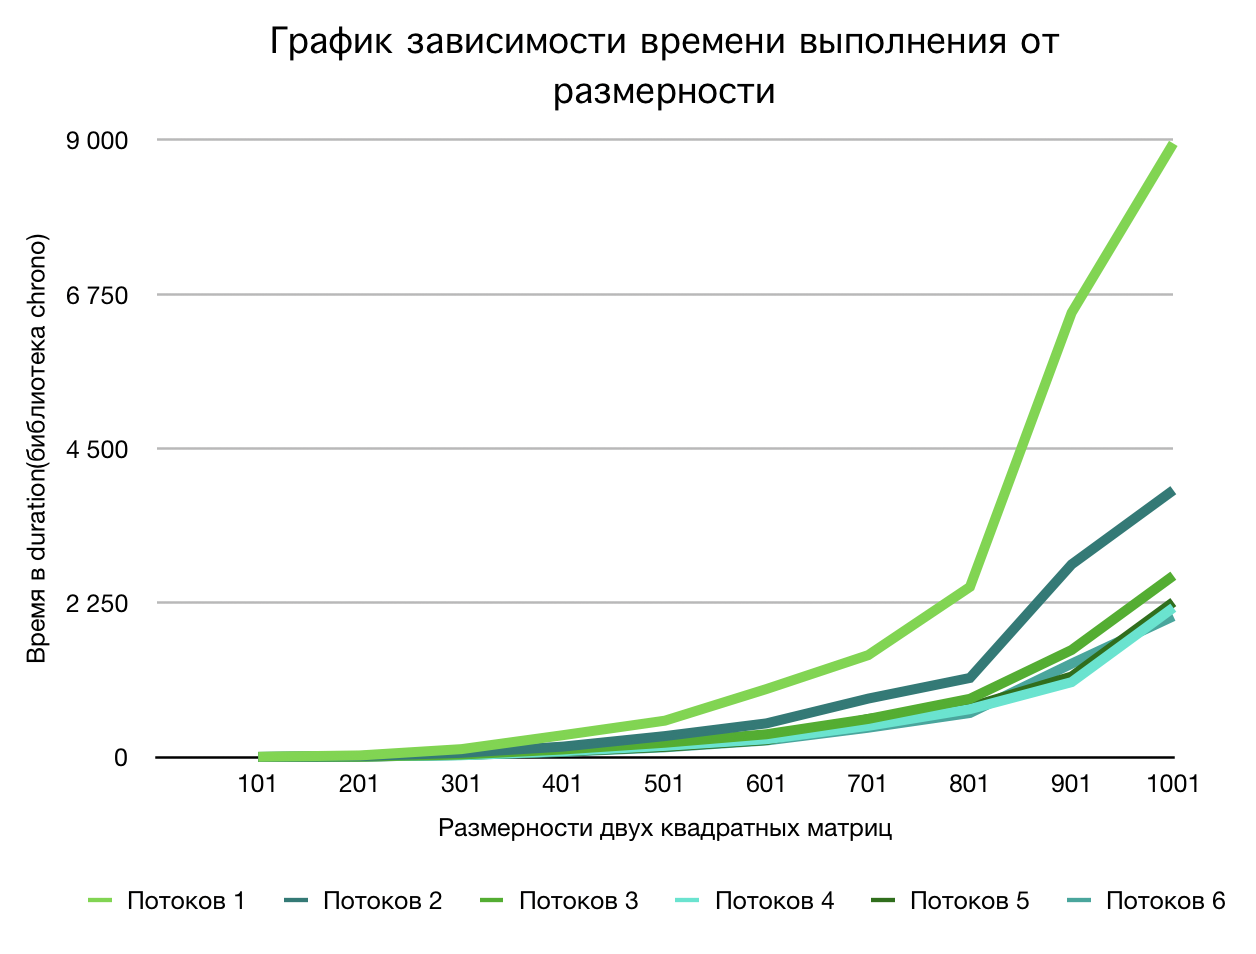
\includegraphics[scale=0.75]{table2}
		\caption{График зависимости времени работы однопоточной и многопоточных версий алгоритма для нечетной размерности матриц}
		\label{fig:image}
	\end{figure}

	\begin{table}[ht!]
		\caption{Время работы программы для 7 и 8 потоков}
		\label{table3}
		\begin{center}
			\begin{tabular}{|c|c|c|}
				\hline
				\bf{Размерность матриц} & \bf{Поток 7} & \bf{Поток 8} \\\hline
				
				$100$ & $1$ & $1$\\\hline
				
				$200$ & $7$ & $6$\\\hline
				
				$300$ & $26$ & $26$\\\hline
				
				$400$ & $70$ & $66$\\\hline
				
				$500$ & $132$ & $126$\\\hline
				
				$600$ & $218$ & $210$\\\hline
				
				$700$ & $410$ & $370$\\\hline
				
				$800$ & $595$ & $581$\\\hline
				
				$900$ & $1133$ & $937$\\\hline
				
				$1000$ & $1356$ & $1482$\\\hline
			\end{tabular}
		\end{center}
	\end{table}

	Из данных графиков видно, что присутствие хотя бы двух потоков в несколько раз эффективнее, в сравнению с однопоточной реализацией алгоритма. Разница по времени выполнения в многопоточной реализации алгоритма не зависит от четной или нечетной размерности матриц. Самое опитмальное количество потоков для реализации данного алгоритма - 4, из-за того что на восьми потоках разниц не существенна. 
	\newpage
	
	\section{Вывод}
	
	\hspace{0.6cm}В данном разделе было проведено исследование однопоточной и многопоточных версий алгоритма. Приведены графики зависимостей времени работы алгоритма от размерности матриц.
	
	\vspace{0.3cm}Среди всех версий алгоритма самыми лучшим оказались версии, где задействовалось не менее четырех потоков. Многопоточная версия алгоритмов показала хороший реазультат относительно однопоточной версии: восьмипоточная реализация алгоритма эффективней однопоточной на 400\% при размерности матриц равной 1000.

	\newpage

	\chapter{Заключение}
	\addcontentsline{toc}{chapter}{Заключение}
		\vspace{-0.6cm}\hspace{0.5cm}В ходе выполнения данной лабораторной работы были изучены и реализованы различные алгоритмы перемножения матриц. В аналитической части было приведено описание алгоритмов. В конструкторской части были представлены блок-схемы алгоритмов. Также был выполнен расчет сложности алгоритмов. В экспериментальной части проведен сравнительный анализ временных затрат, после которого была выявлена ощутимая эффективность многопоточного программирования по отношению к стандартному, однопоточному. 
		
		\vspace{0.3cm}На матрицы размерности 1000х1000 результаты оказались следующими:
	\begin{itemize} 
		\item Эффективность 1 потока к 2 потокам составила 240\%.
		\item Эффективность 1 потока к 4 потокам составила 490\%.
		\item Эффективность 1 потока к 6 потокам составила 700\%.
		\item Эффективность 1 потока к 8 потокам составила 720\%.
	\end{itemize}
	
	\newpage

\begin{thebibliography}{3}
	\bibitem{Sulsky1994}
	Энтони Уильямс Параллельное программирование на С++ в действии. Практика разработки многопоточных программ.
	\bibitem{bmstu}
	Многопоточность [Электронный ресурс]. - Режим доступа: https://ru.bmstu.wiki/Многопоточность, свободный. (Дата обращения: 20.11.2019 г.)
	\bibitem{Volkova}
	Многопоточность [Письменный ресурс]. - Семинар по анализу алгоритмов. (Дата обращения: 19.11.2019 г.)
\end{thebibliography}
\end{document}

\end{document}
